% !TeX root = RJwrapper.tex
\title{Capitalized Title Here}
\author{by Author One and Author Two}

\maketitle

\abstract{%
An abstract of less than 150 words.
}

\hypertarget{real-rata-and-simulations}{%
\subsection{Real Rata and Simulations}\label{real-rata-and-simulations}}

\hypertarget{boston-housing-data}{%
\subsubsection{Boston Housing data}\label{boston-housing-data}}

\begin{Schunk}
\begin{Sinput}
# install.packages("quantreg","KernSmooth")
# install.packages(pkgs= "https://github.com/zzz1990771/siqr/raw/master/siqr_0.1.0.zip", repos = NULL, type = "win.binary")
library(siqr)
\end{Sinput}
\begin{Soutput}
#> Loading required package: quantreg
\end{Soutput}
\begin{Soutput}
#> Loading required package: SparseM
\end{Soutput}
\begin{Soutput}
#> 
#> Attaching package: 'SparseM'
\end{Soutput}
\begin{Soutput}
#> The following object is masked from 'package:base':
#> 
#>     backsolve
\end{Soutput}
\begin{Soutput}
#> Loading required package: KernSmooth
\end{Soutput}
\begin{Soutput}
#> KernSmooth 2.23 loaded
#> Copyright M. P. Wand 1997-2009
\end{Soutput}
\begin{Sinput}
#load data from MASS
library(MASS)
#help(Boston)
medv<- Boston$medv
RM <- Boston$rm
logTAX <- log(Boston$tax)
PTRATIO <- Boston$ptratio
logLSTAT <- log(Boston$lstat)

X <- cbind(RM,logTAX,PTRATIO,logLSTAT)
y0<-medv - mean(medv)

beta0 <- NULL
tau.vec <- c(0.25,0.5,0.75)
est.coefficient <- matrix(NA, nrow = length(tau.vec), ncol = 5)
est.coefficient[,1] <- tau.vec
for (i in 1:length(tau.vec)){
  est <- siqr(y0,X,beta.initial = beta0, tau=tau.vec[i],maxiter = 20,tol = 1e-6)
  est.coefficient[i,2:5] <- est$beta
}
colnames(est.coefficient) <- c("quantile tau",colnames(X))
est.coefficient
\end{Sinput}
\begin{Soutput}
#>      quantile tau        RM     logTAX     PTRATIO   logLSTAT
#> [1,]         0.25 0.3365972 -0.5237661 -0.06832911 -0.7795528
#> [2,]         0.50 0.3108555 -0.4282412 -0.06633865 -0.8459181
#> [3,]         0.75 0.2427424 -0.1999916 -0.07720527 -0.9461072
\end{Soutput}
\end{Schunk}

\begin{Schunk}
\begin{Sinput}
est.tau25 <- siqr(y0,X,beta.initial = NULL, tau=0.25)
plot.siqr(est.tau25,bootstrap.interval = TRUE)
\end{Sinput}

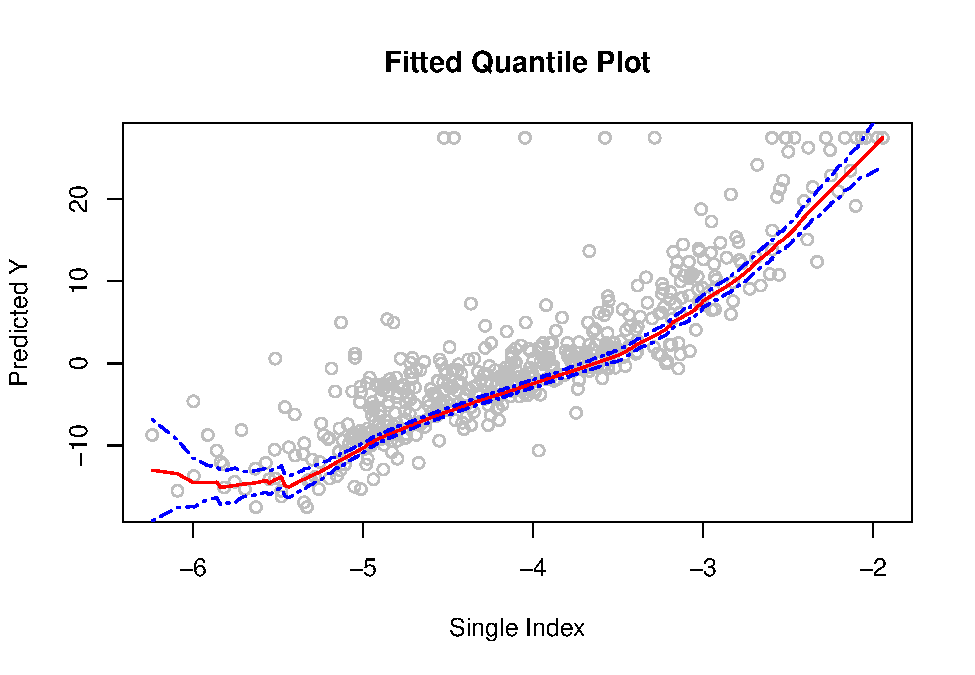
\includegraphics{siqr_files/figure-latex/unnamed-chunk-2-1} \end{Schunk}

\begin{Schunk}
\begin{Sinput}
est.tau50 <- siqr(y0,X,beta.initial = NULL, tau=0.5)
plot.siqr(est.tau50,bootstrap.interval = TRUE)
\end{Sinput}

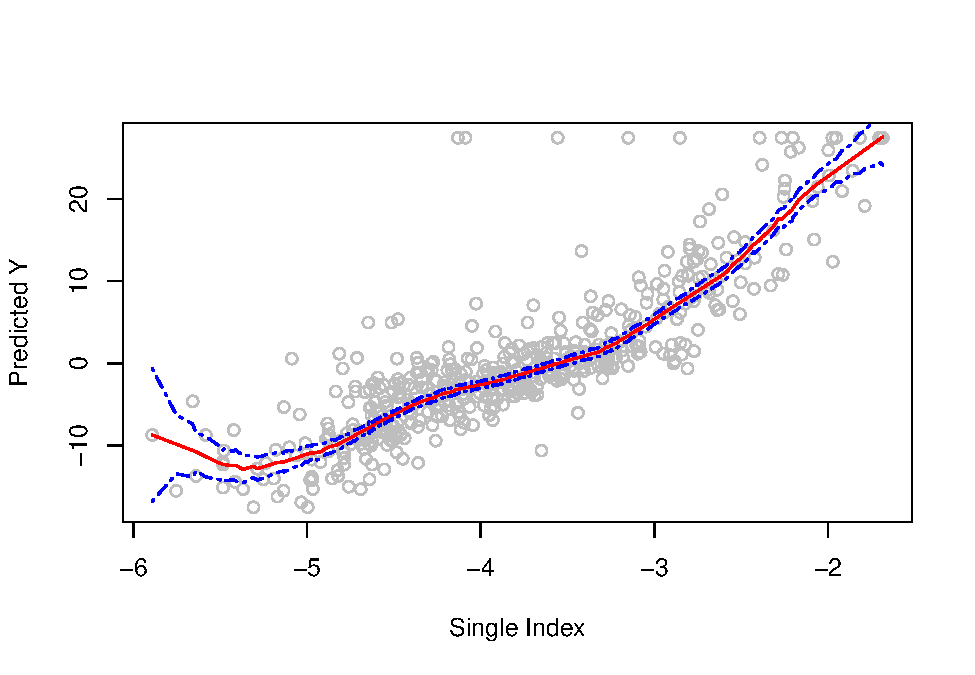
\includegraphics{siqr_files/figure-latex/unnamed-chunk-3-1} \end{Schunk}

\begin{Schunk}
\begin{Sinput}
est.tau75 <- siqr(y0,X,beta.initial = NULL, tau=0.75)
plot.siqr(est.tau75,bootstrap.interval = TRUE)
\end{Sinput}

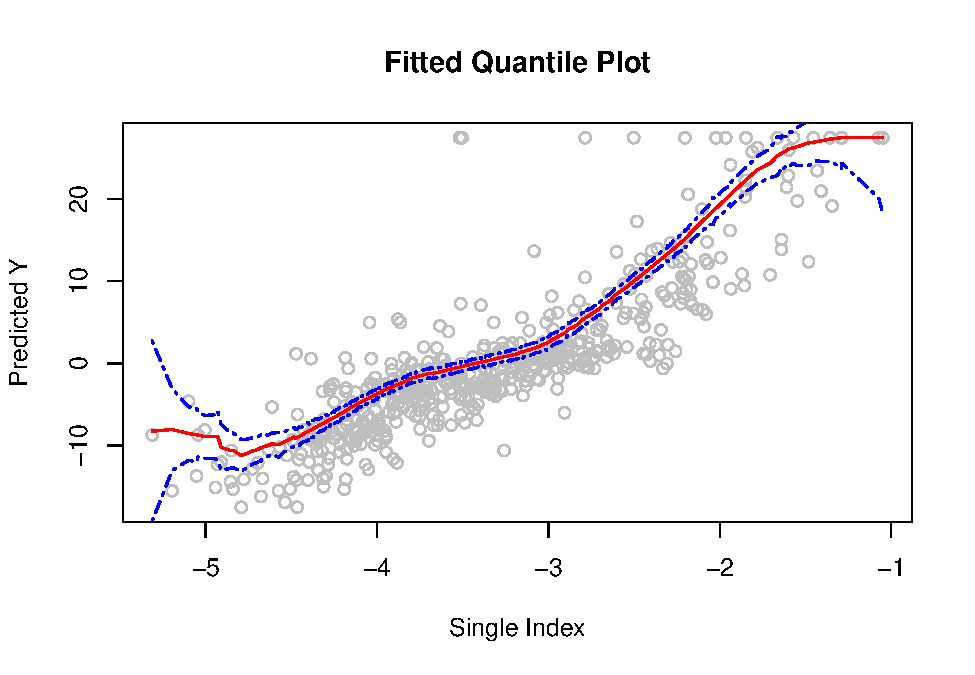
\includegraphics{siqr_files/figure-latex/unnamed-chunk-4-1} \end{Schunk}

\hypertarget{simulation}{%
\subsubsection{Simulation}\label{simulation}}

\hypertarget{setting-1}{%
\paragraph{Setting 1}\label{setting-1}}

\begin{Schunk}
\begin{Sinput}
n <- 400
beta0 <- c(1, 1, 1)/sqrt(3)
n.sim <- 200
tau.vec <- c(0.25,0.5,0.75)
tau <- tau.vec[1]

data <- generate.data(n, true.theta=beta0, setting = "setting1",ncopy = n.sim)

#paralell 
library(parallel)
library(foreach)
cl<- makeCluster(12)
doParallel::registerDoParallel(cl)
sim.results.50 <- foreach(m = 1:n.sim,.combine = "rbind") %dopar% {
  X <- data$X
  Y <- data$Y[[m]]
  est <- siqr(Y, X, beta.initial = c(2,1,0), tau=0.5,maxiter = 30,tol = 1e-8)
  if(est$flag.conv == 0){
    return(NULL)
  }else{
    return(est$beta)
  }
}

sim.results.25 <- foreach(m = 1:n.sim,.combine = "rbind") %dopar% {
  X <- data$X
  Y <- data$Y[[m]]
  est <- siqr(Y, X, beta.initial = c(2,1,0), tau=0.25,maxiter = 30,tol = 1e-8)
  if(est$flag.conv == 0){
    return(NULL)
  }else{
    return(est$beta)
  }
}
sim.results.75 <- foreach(m = 1:n.sim,.combine = "rbind") %dopar% {
  X <- data$X
  Y <- data$Y[[m]]
  est <- siqr(Y, X, beta.initial = c(2,1,0), tau=0.75,maxiter = 30,tol = 1e-8)
  if(est$flag.conv == 0){
    return(NULL)
  }else{
    return(est$beta)
  }
}
stopCluster(cl)
\end{Sinput}
\end{Schunk}

\begin{Schunk}
\begin{Sinput}
sim.results.25 <- readRDS("./sim1.results25.RDS")
sim.results.50 <- readRDS("./sim1.results50.RDS")
sim.results.75 <- readRDS("./sim1.results75.RDS")
\end{Sinput}
\end{Schunk}

\begin{Schunk}
\begin{Sinput}
boxplot(data.frame((sim.results.25)), outline=T,notch=T,range=1,main = "Boxplots of Coefficient Estimates, tau = 0.25",horizontal = F,
names=c(expression(hat(beta)[1]),expression(hat(beta)[2]),expression(hat(beta)[3])))
\end{Sinput}

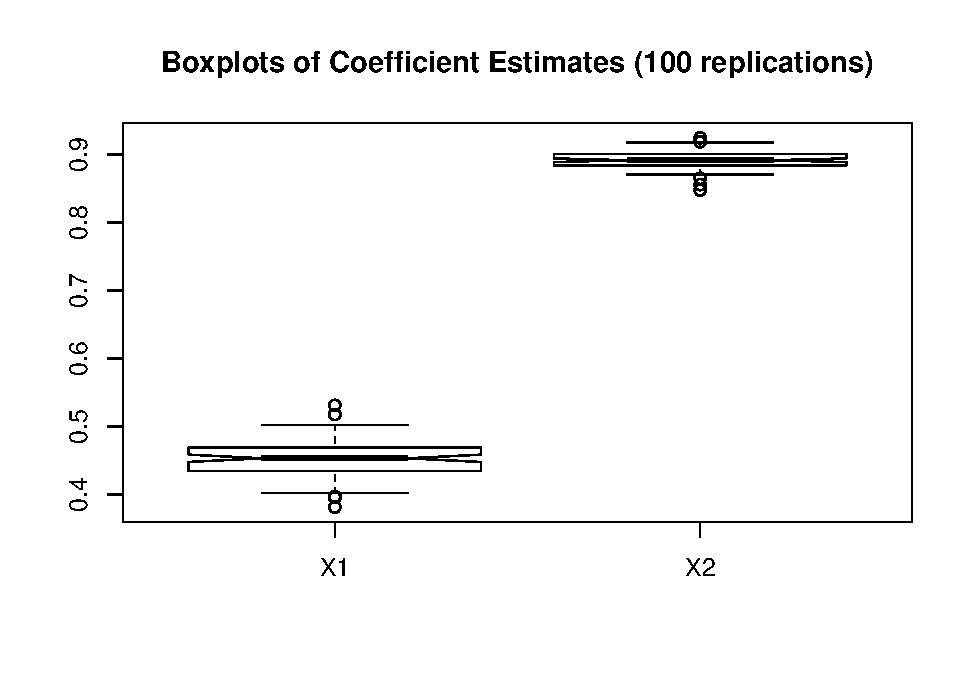
\includegraphics{siqr_files/figure-latex/unnamed-chunk-7-1} \end{Schunk}

\begin{Schunk}
\begin{Sinput}
boxplot(data.frame((sim.results.50)), outline=T,notch=T,range=1,main = "Boxplots of Coefficient Estimates, tau = 0.25",horizontal = F,
names=c(expression(hat(beta)[1]),expression(hat(beta)[2]),expression(hat(beta)[3])))
\end{Sinput}

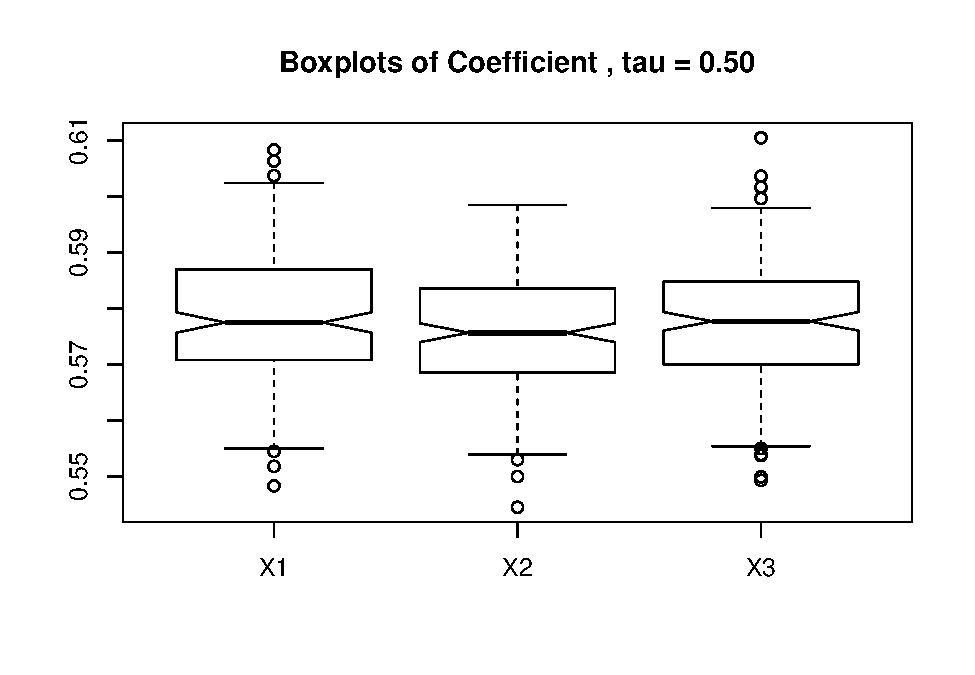
\includegraphics{siqr_files/figure-latex/unnamed-chunk-8-1} \end{Schunk}

\begin{Schunk}
\begin{Sinput}
boxplot(data.frame((sim.results.75)), outline=T,notch=T,range=1,main = "Boxplots of Coefficient Estimates, tau = 0.25",horizontal = F,
names=c(expression(hat(beta)[1]),expression(hat(beta)[2]),expression(hat(beta)[3])))
\end{Sinput}

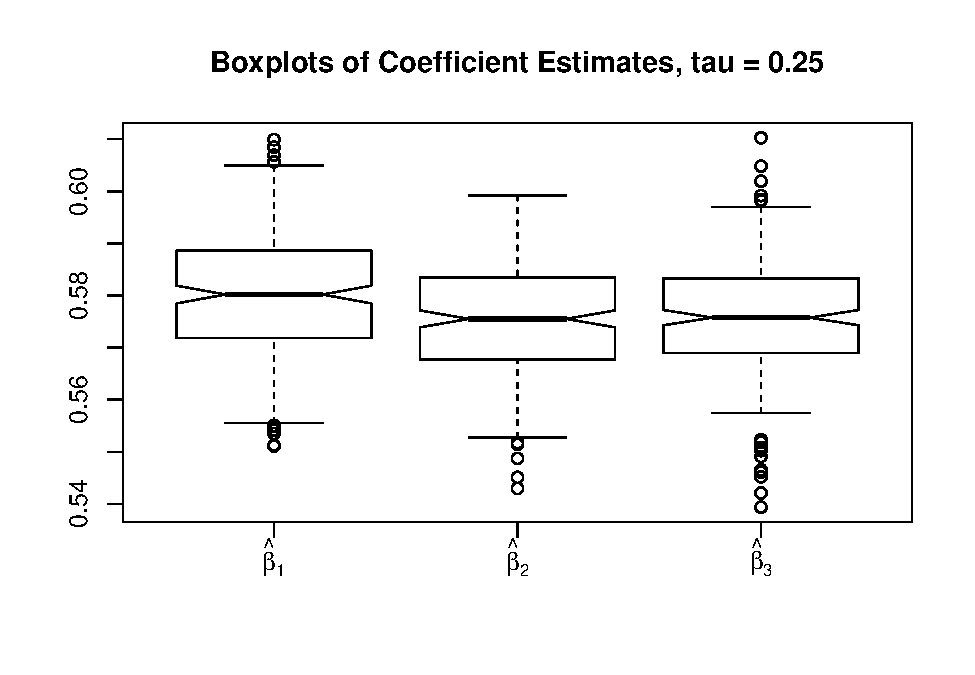
\includegraphics{siqr_files/figure-latex/unnamed-chunk-9-1} \end{Schunk}

\begin{Schunk}
\begin{Sinput}
est.sim.05 <- siqr(data$Y[[1]],data$X,beta.initial = NULL, tau=0.5)
plot.siqr(est.sim.05,bootstrap.interval = TRUE)
\end{Sinput}
\end{Schunk}

\hypertarget{setting-3}{%
\paragraph{Setting 3}\label{setting-3}}

\begin{Schunk}
\begin{Sinput}
n <- 400
beta0 <- c(1, 2)/sqrt(5)
n.sim <- 100
tau <- 0.5

data <- generate.data(n, true.theta=beta0, setting = "setting3",ncopy = n.sim)

#paralell 
library(parallel)
library(foreach)
cl<- makeCluster(12)
doParallel::registerDoParallel(cl)
sim.results <- foreach(m = 1:n.sim,.combine = "rbind") %dopar% {
  X <- data$X
  Y <- data$Y[[m]]
  est <- siqr(Y, X, beta.initial = NULL, tau=tau,maxiter = 30,tol = 1e-8)
  est$beta
}
\end{Sinput}
\end{Schunk}

\begin{Schunk}
\begin{Sinput}
tau <- 0.5
sim.results <- readRDS("./sim.results.RDS")
est.mean <- c(tau,apply(sim.results,2,mean))
names(est.mean) <- c("tau","beta1.hat","beta2.hat")
est.mean
\end{Sinput}
\begin{Soutput}
#>       tau beta1.hat beta2.hat 
#> 0.5000000 0.4515909 0.8917233
\end{Soutput}
\end{Schunk}

\begin{Schunk}
\begin{Sinput}
est.se <- c(tau,apply(sim.results,2,sd))
names(est.se) <- c("tau","beta1.se.hat","beta1.se.hat")
est.se
\end{Sinput}
\begin{Soutput}
#>          tau beta1.se.hat beta1.se.hat 
#>   0.50000000   0.02682211   0.01359602
\end{Soutput}
\end{Schunk}

\begin{Schunk}
\begin{Sinput}
boxplot(data.frame((sim.results)), outline=T,notch=T,range=1,main = "Boxplots of Coefficient Estimates, Example 2",horizontal = F,
names=c(expression(hat(beta)[1]),expression(hat(beta)[2])))
\end{Sinput}

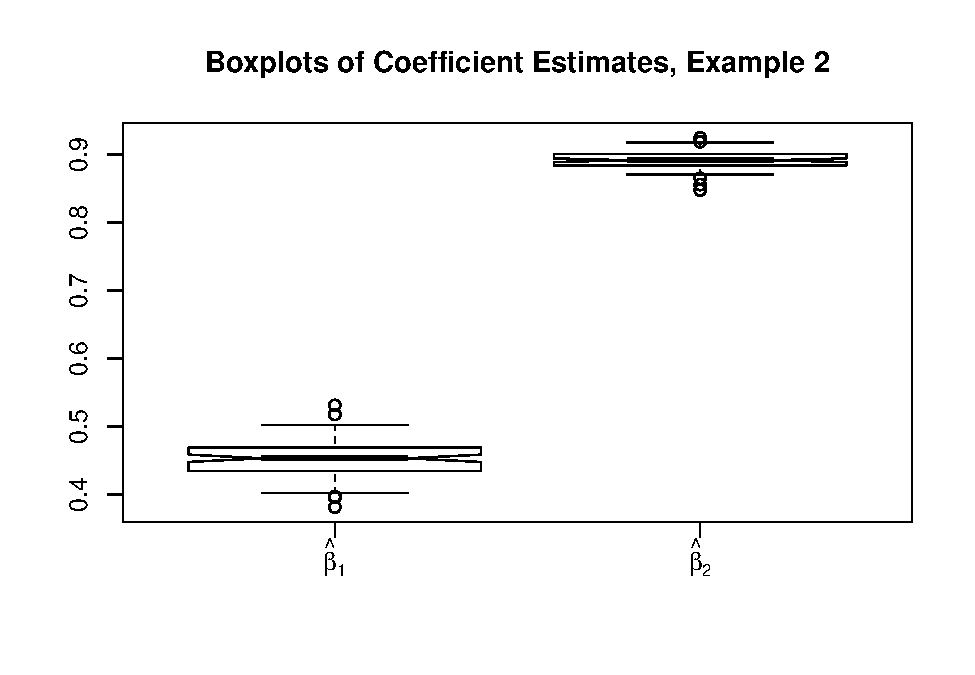
\includegraphics{siqr_files/figure-latex/unnamed-chunk-14-1} \end{Schunk}

\begin{Schunk}
\begin{Sinput}
n <- 400
beta0 <- c(1, 2)/sqrt(5)
n.sim <- 100
tau <- 0.5
data <- generate.data(n, true.theta=beta0, setting = "setting3",ncopy = 2)
est.sim.05 <- siqr(data$Y[[1]],data$X,beta.initial = NULL, tau=0.5)
plot.siqr(est.sim.05,bootstrap.interval = TRUE)
\end{Sinput}

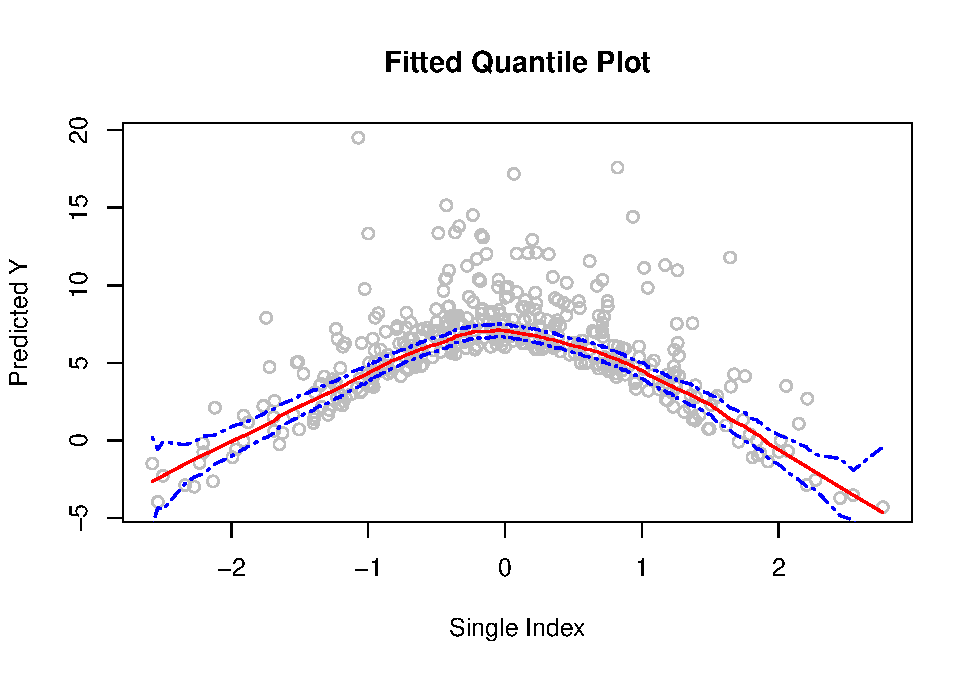
\includegraphics{siqr_files/figure-latex/unnamed-chunk-15-1} \end{Schunk}

\begin{Schunk}
\begin{Sinput}
Sys.sleep(100)
\end{Sinput}
\end{Schunk}

\bibliography{RJreferences}


\address{%
Author One\\
Affiliation\\%
line 1\\ line 2\\
%
%
%
\href{mailto:author1@work}{\nolinkurl{author1@work}}%
}

\address{%
Author Two\\
Affiliation\\%
line 1\\ line 2\\
%
%
%
\href{mailto:author2@work}{\nolinkurl{author2@work}}%
}
